\documentclass{article}

\usepackage{tikz}

\begin{document}

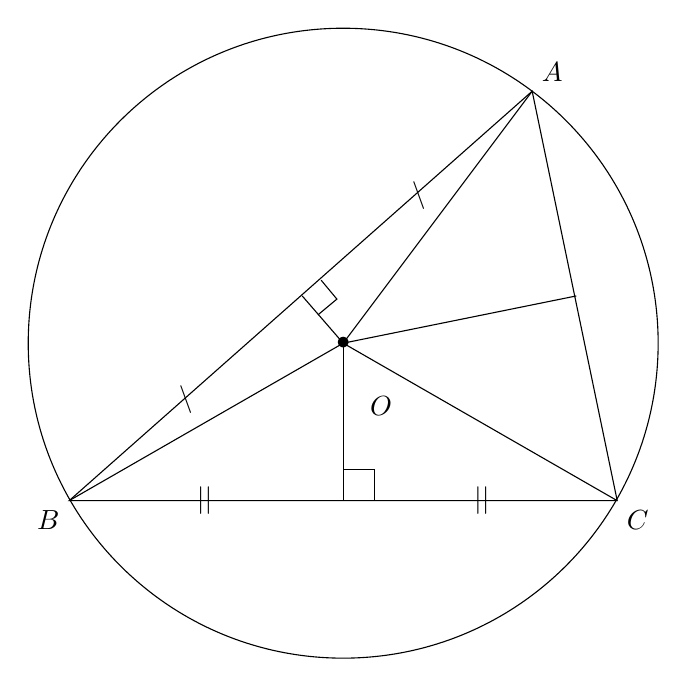
\begin{tikzpicture}[scale=4]
    \draw (0.87,-0.5) node[below right]{$C$}
       -- (0.6,0.8) node[above right]{$A$} 
       -- (-0.87,-0.5) node[below left]{$B$}--cycle ;
    \draw (0,0) edge (0,-0.5)
                edge (0.74, 0.15)
                edge (-0.13, 0.15)
                edge (0.87, -0.5)
                edge (0.6,0.8)
                edge (-0.87,-0.5);
    \draw (0,0) circle (1);
    \draw (0,0) node {$\bullet$} + (0.12,-0.2) node{$O$};
    \draw (0.24, 0.47) node {\textbackslash};
    \draw (-0.5, -0.18) node {\textbackslash};
    \draw (-0.44, -0.5) node{$||$} ;
    \draw (0.44, -0.5) node{$||$} ;
    \draw (0.1,-0.5) -- (0.1,-0.4) -- (0,-0.4) ;
    \draw (-0.08,0.09) -- (-0.02,0.14) -- (-0.07,0.2) ;
\end{tikzpicture}

\end{document}
